\documentclass[a4paper,12pt]{book}
\usepackage[margin=1in]{geometry} % 设置边距,符合Word设定
\usepackage{ctex} %导入中文包
\title{人造语言Arka考}
\author{亿年-二孤旋\quad 搬运\quad  译 }

\date{2021}
\usepackage{graphicx}
\usepackage{float}
\usepackage[utf8]{inputenc}

\usepackage{geometry} %设置页边距的包

\usepackage{pdfpages} %本文最重要的一个包,就是将PDF文件加入到封面位置
\setmainfont{Times New Roman}%调节IPA输入兼容性
\usepackage{hyperref}
\hypersetup{hidelinks,
	colorlinks=true,
	allcolors=black,
	pdfstartview=Fit,
	breaklinks=true
}
%\usepackage{movie15}
\usepackage{media9}
\usepackage{bbding}
\usepackage{attachfile2}%这个对中文,xelatex顶用
%\usepackage[colorlinks,linkcolor=blue]{hyperref}
\usepackage{appendix}%附录
\usepackage{color}%字体颜色
\newcommand{\emoji}[1]{
\begin{figure}[H]
\includegraphics{pngs/#1.png}
\end{figure}
}
\geometry{left=2.5cm,right=2cm,top=2.54cm,bottom=2.54cm} %设置书籍的页边距
\begin{document}

\maketitle
% 插入封面
%\include{.Tex_files/cover} %此处是调用外置的定义好的封面文件

% 插入摘要
\frontmatter
\noindent そは きえゆくものか\\
ほろびに そのみをゆたね\\
なをしるものもと だえ\\
しんさえも うしなわれ\\
いまはとて がんさぶるみも\\
あわれや あわれや\\

\textit{------Calling,凋叶棕}\\

幻想,一切生命最终的归宿,呼唤着,引诱着,被遗忘的种种存在.即便是
人造语言这般幻想的产物,也不免被嘈杂的声音淹没,最终归于幻想的虚无.
我偶然发现Arka这以页面后,旋即被她悠久的历史,广大的体量所吸引.
又不忍她又无人问津,苦苦等待下一个踏入圣域的旅人,因此把网页上的全部内容
截取下来,再翻译,整理成文档,希望更多的人能够看见她,参与到她的创作和流通中去.

我自知能力有限,不能完整地展现原著的风采,于是就把原著的链接放在这里,
大家可以直接去看,如果我翻得有什么问题,也请读者批评指正.

官网(日,英,韩语):\url{http://conlinguistics.org/arka/e\_index.html}

%\include{./Tex_files/chapter中文摘要}
%\include{./Tex_files/chapter英文摘要}
% 插入目录
\tableofcontents% 插入正文
\mainmatter
\part{综述}
\chapter{Arka简要介绍}
Arka是一种人造语言.1991年始,她从零开始设计,处处都可以见到精巧的构思,在人文科学,哲学和语言学方面都有涉及.
现在她已经有一万六千余词,并且有自己的世界-Kaldia.

作为一门先验语,她的思路和世界语迥然不同,没有从英语,日语,汉语等现有语言做任何的借词.
她的所有词汇,都是,从草稿开始,进行词源的衍生和流变,一步一步发展起来的.
要知道,大多数创作者无法支撑这样一个庞大的先验语系,所以多采用后验方法构词,或是只建立一个很小的先验词汇表.
另外的一系是走工程语言的路线,像是John Wilkins的"真字".
\footnote{Real Character,由John Wilkins(1614-1672)建立的一门先验语,
其方向是成为一门世界辅助语,供学术和外交使用.
详见
\textattachfile{attachfiles/an essay towards a real character.7z}
{An Essay Towards a Real Character, and a Philosophical Language (London, 1668)}
这本书实在是太老又太大,译者无暇仔细阅读,但是将HTML格式的书打包成7z附于书中,供有心人参考.
}
能到Arka这样一万六千余词的规模,囊括世界观和文化细节\footnote{甚至有专门的章节讲述魔法的进化历程},实属不易.

Arka是一门在Kaldia讲述的艺术语,但也可以被地球人言说.
官网的建立者就是讲着日语,芬兰语,爱沙尼亚语,法语和德语等的总计30余人,
学习者更是遍布日,韩,中,英,美诸国.
至现在,学习者数量已有三倍的增长.


\section{开始}
读者可以看``诗姬和悠姬的一点Arka动画'',这是大概10分钟的动画.
\footnote{视频在YouTube上,官网的播放器已经不顶用了}
没有时间或者不方便的话,可以看这一章介绍的图.
\begin{figure}[H]
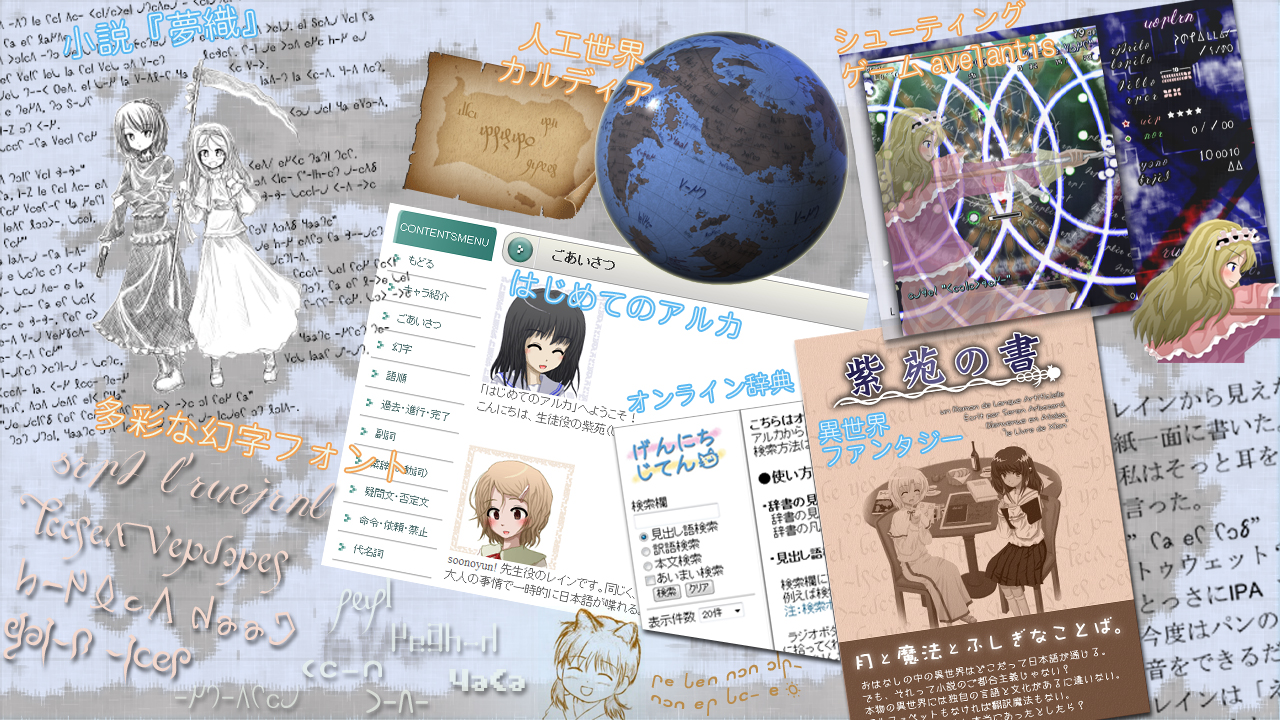
\includegraphics[width=1\textwidth]{ARKA/leis.jpg}
\end{figure}
有余裕的话,还可以看看\href{http://www44.atwiki.jp/conlang_arka/pages/1.html}{ARKA的特性}和
\textattachfile{attachfiles/語法論-人工言語の見えない心臓.pdf}{语法论-人造语言无形的心脏(日语)}
,我们也推荐\href{http://conlinguistics.org/arka/e_study_kit.html}{给初心者的指南}.

\small{
译者的话:

我翻译了初学者课程的第一部分,就是之后章节Lein的课程.但是整个网站的内容太多,我难以完全翻译.
希望有心人可以接续我的愿望.这本书以latex制成,等到网好的时候我会把所有的文档放在github上.
大家都可以来参与翻译.

\quad --亿年-二孤旋
}
\section{相关网页}

%arka维基:\url{https://arka.fandom.com/wiki/ARKA_Wiki}

Arka词典(Arka<->日语):\url{http://mindsc.ape.jp/klel/}

\part{Lein的课程}
\chapter[问候]{问候}
%\chapter[短标题显示在页面]{长标题显示在目录}

% {\small\textit{
% \quad Sors de l'enfance, ami réveille toi!\newline
% \quad \quad —Jean Jacques Rousseau.}
% \footnote{Ekster el infaneco,amiko veku!}
% \\}

\emoji{x_sena}
% \begin{figure}[h]
% 
\includegraphics{pngs/x_sena.png}
% \label{x_sena}
% \end{figure}

欢迎来到Lein的课程!

大家好, 我是学生紫苑. 现在17岁,在上高二.

\emoji{l_sena}

Soonoyun [so:nɔjɯn]! 我叫Lein,是你的老师. 我也是Arbazard中学的学生.
\footnote{这几位女生是``紫苑之书''中的主人公,Nias Avelantis制作了立绘(还包含以后会介绍的Alia和Arshe).感谢他的贡献}

我本来不该说汉语的,但是编辑叫我说我就说吧. :)

\emoji{x_knoos}

那个,你说的第一个词是啥? 额... soonoyun ?

还有Arbazard又是哪?我在世界地图上没找到.

\emoji{l_rana}

Soonoyun 意思是``你好''. 它可以指代早上好,中午好和晚上好.有用吧?
Arbazard是Atolas的一个国家,而Atolas是我居住的星球. 我们国家通行的语言就是Arka.

\emoji{x_naki}

Arka不是地球上的语言吧?怪不得我没见过这些字母.
\begin{figure}[H]
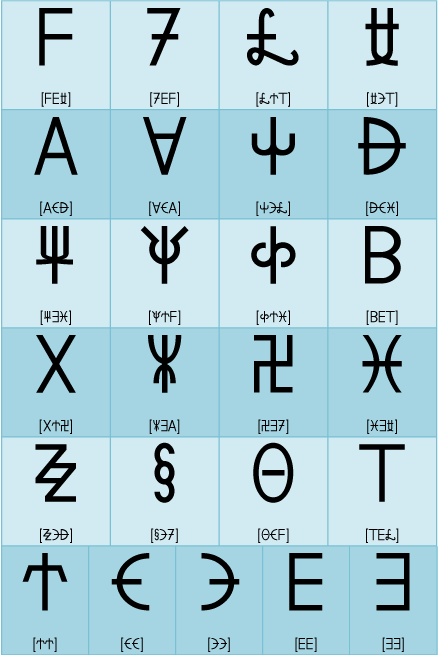
\includegraphics[width=0.5\textwidth]{ARKA/klandi.png}
\end{figure}
\emoji{l_deyu}

这些字母是幻字的大写字母.
20个是辅音,5个是元音,总共有25个.
在Arka中,幻字被叫做hacm.

\emoji{x_lek}

这也忒难记了吧!

我可能记得住E 和 F, but...

\emoji{l_ket}

其实, 我们很少用大写字母,你只要记住这些小写字母就行了.
\begin{figure}[H]
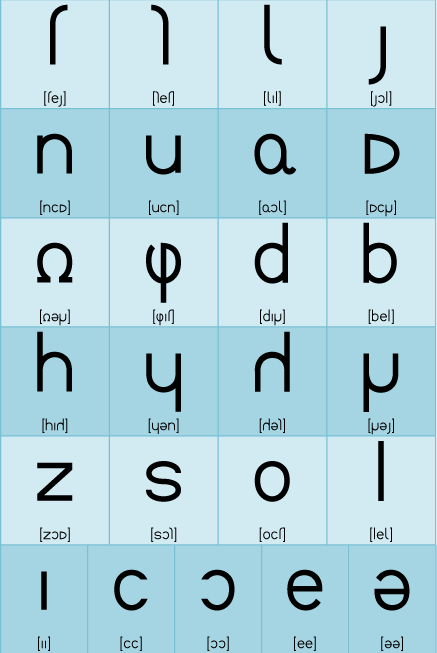
\includegraphics[width=0.5\textwidth]{ARKA/lemal.png}
\end{figure}
\emoji{x_tisse}

这样啊,那说不定能行.所有字母都只有一画,有些字母还和拉丁字母很像.
幻字来自别的世界,但某种程度上还真是相似啊.

\emoji{l_rana}

你发现了奇妙的东西呢.不过关于字母的文章现在对你来说还太难.

\emoji{x_lo}

小写字母虽说简单,但我还是要花点功夫记.现在嘛,我要用拉丁字母转写Arka.
在我熟悉字母表之前,我还是先看这个语言的转写版凑合.
\begin{figure}[H]
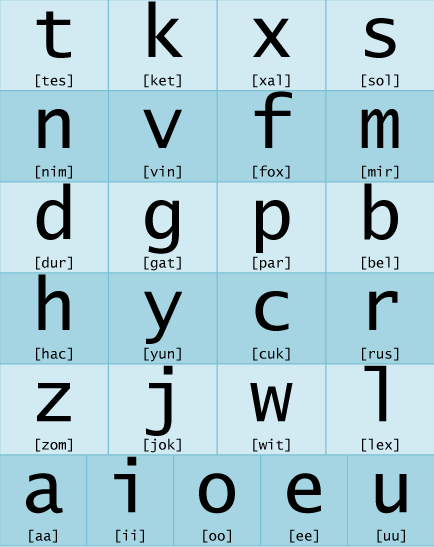
\includegraphics[width=0.5\textwidth]{ARKA/tenxa.png}
\end{figure}
\emoji{x_lo}

转写的Arka大部分都还行.就是``x''和``c''发音有些奇怪.``x''发[ʃ](像``shop''里的``sh''),``c''是卷舌的 R (像西班牙词``burro''里的``rr'').

So, ``c''是齿槽颤音[r], whereas ``r''是齿槽近音[ɹ].

其他的字母...? ``y'' ([j])像"yes."的``y'', ``j'' ([ʒ])像``vision''的``s''.``h''([h])像``happy''里的``h'', ``w'' ([w])像``wise''的``w''.

\emoji{l_rana}

熟悉幻字的时候就用拉丁转写吧. ``tx'' ([tʃ])像  ``church''的``ch'',``ts''发``cats''的``ts''.

幻字是专门书写Arka的,所以用来写Arka就很有效.一步一步来嘛.

很多字母都相互对称;我小时候就经常把``tes''混成``ket''.长大了就分的清了,就像你区分``d''和``b''一样.

\emoji{x_sena}

看来我应该一步一步来,多动笔写写.
不管咋样,我该练练转写啦.\textbf{``x''发``shop''的``sh'', ``c''发西班牙语``burro''的``rr''.}
说干就干!

%"([a-z]+)"
%``$1''



\chapter[幻字]{幻字}
%\chapter[短标题显示在页面]{长标题显示在目录}

% {\small\textit{
% \quad Sors de l'enfance, ami réveille toi!\newline
% \quad \quad —Jean Jacques Rousseau.}
% \footnote{Ekster el infaneco,amiko veku!}
% \\}


\emoji{l_sena}

Soonoyun(你好)! 是我,Lein.今天我们来上第二课吧.
紫苑啊,你记住幻字的拉丁转写了吗?

\emoji{x_asex}

那是.我现在看转写词没啥问题,驾驶碰到"x"和"c"要小心. 
"x"发音像"shop"的"sh","c" 像西班牙语"burro"里的"rr".
把"c"当做[r]有点怪,但是我不想依赖别的例子去记它.
"シ"在Arka中写作"xi",所以我的名字在Arka里写作"Xion",不是"Shion".


\emoji{l_iks}

你别把xion读成ksion了,OK?

\emoji{x_seernik}

Xion... 我想到一个播放器\footnote{Zeon,瑞翁电器} :)

\emoji{l_niit}

先别管讲笑话,现在发音如何了?

\emoji{x_nal}
还是不习惯.但我会尽力去做的
让我试试这样行不行.顺便把字母表写下来.

% \includemedia[label=lettersong,flashvars={source=ARKA/hacm.mp3},
% transparent,
% passcontext %show VPlayer's right-click menu
% ]{}{APlayer.swf}\\
% \mediabutton[
% mediacommand=lettersong:play
% ]{\fbox{发音}}
% \mediabutton[
% mediacommand=lettersong:pause
% ]{\fbox{暂停}}

\begin{figure}[H]
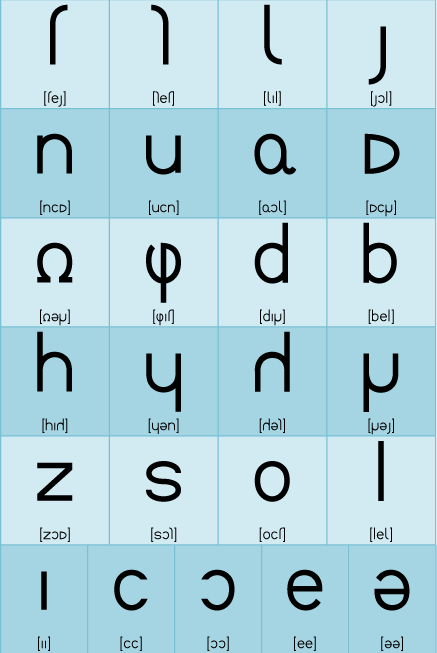
\includegraphics[width=0.5\textwidth]{ARKA/lemal.png}
\end{figure}
Yeah,这就挺不错的(=°ω°)ノニャン♪

"c"就像"burro"里的"rr",但是女生喜欢像日语的"r"一样发音就像"ramen"([ɾaːmen]). 
学术点的讲,就是齿龈闪音.

接下来,来听听\textattachfile{ARKA/hacm.mp3}
{字母歌}吧.
%"([a-z]+)"
%``$1''
\chapter[语序]{语序}
%\chapter[短标题显示在页面]{长标题显示在目录}

% {\small\textit{
% \quad Sors de l'enfance, ami réveille toi!\newline
% \quad \quad —Jean Jacques Rousseau.}
% \footnote{Ekster el infaneco,amiko veku!}
% \\}


\emoji{l_sena_deyu}
今天我们来学习Arka的语序吧!

汉语里,像``黑猫''这样的词,形容词在名词前面,但是在Arka里,你应该说``猫-黑.''


\emoji{x_loki}
你说...像法语那样? ``黑猫''在法语里叫做``chat noir''.形容词``noir''在名词``cat''后面.

在Arka里,就说``ket (猫) ver (黑)'',对吧?

明白了,形容词在名词后面.那么,你们是如何造句子的呢?


\emoji{l_niit}
就像汉语那样.

举个栗子,说``紫苑看到Lein,''你就像``紫苑'' + ``看'' + ``Lein''这样拼起来.你知道的,``主语'' + ``谓语'' + ``宾语.''

``看''在Arka里叫``in'',所以你要说``紫苑看到Lein,''就说:``xion in lein.''


\emoji{x_pil}
这就叫SVO.
在这一点上,Arka和汉语,英语都很像呢.


\emoji{l_deyu}
那么问题来了.
你怎么表达``大狗看小猫''呢?

单词: 大 = kai, 小 = lis, 狗 = oma, 猫 = ket,看 = in


\emoji{x_lo}
形容词在名词后面,so``大狗''就是``oma kai'',``小猫''就是``ket lis.''

语序是SVO,那么...

``Oma kai in ket lis,''这样?


\emoji{l_uni}
好!

嘿呀,你会用Arka造句子了.(v\^{}-°)

OK今天结束之前,我们再来看一个问题.

``给''在Arka里是``fit'',苹果是``miik''.So,``Lein给紫苑一个苹果''应该怎么表达?


\emoji{x_fron}
Arka是主-动-宾,就是``lein fit miik.''

慢着,``给紫苑''怎么说?


\emoji{l_niit}
我们用``a''指示目的方.
``A xion''就是``给紫苑''.合起来说就行了.


\emoji{x_tisse}
``A xion''就像英语短语一样,``to Shion''.``A''就像个介词.
所以答案是``lein fit miik a xion,''吗?
这句子还挺长的.我一开始对Arka一无所知,但现在我已经能说出一个句子了.这种不可思议的感觉...
Lein你怎么表达``看了''或者``给了''?


\emoji{l_sena}
我下次就教你Arka的时态. Doova ([doːva] (下次见)) !

%"([a-z]+)"
%``$1''



\chapter[时态]{时态}
%\chapter[短标题显示在页面]{长标题显示在目录}

% {\small\textit{
% \quad Sors de l'enfance, ami réveille toi!\newline
% \quad \quad —Jean Jacques Rousseau.}
% \footnote{Ekster el infaneco,amiko veku!}
% \\}

\begin{figure}[H]
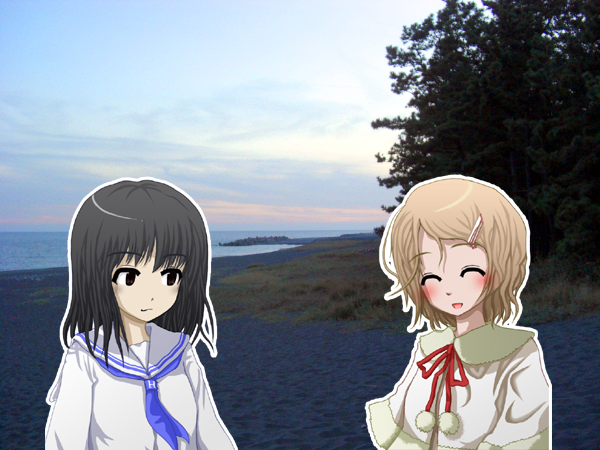
\includegraphics[width=1\textwidth]{ARKA/tier2.jpg}
\end{figure}

Lein: ``我们来海边啦!好-大-的-海-啊!嘿,紫苑,你在干什么?''

紫苑: ``唔...你的腿好细啊.如果我是你的话...''

Lein: ``额...''

紫苑: ``诶~''xion in lein``哦.上次我们学了''紫苑看到了lein.``你也说Arka是SVO型语言''

Lein: ``对对对,形容词在名词后面,记得挺牢的.''


\emoji{x_knoos}
那么,你怎么说``紫苑看到了Lein?''


\emoji{l_sena}
过去时啊,在汉语里,在动词后面加上``了'',在Arka则是``-at''.


\emoji{x_lo}
So,我试着想,``紫苑看到了Lein''就是``xion inat lein,''.

Arka 没有``saw''之类要特殊记的变化,这倒挺简单.没有啥例外吧?


\emoji{l_lo}
我想想...哦哦,动词结尾是元音的话,就不是加``at''而是``-t''.

``Xa''是``在某处'',结尾是元音,所以加 ``-t''.``Xat''就是 ``曾经在某处.''


\emoji{x_loki}
避免元音冲突?

还有``-at''同类型的词缀吗?


\emoji{l_niit}
要表示进行的体
\footnote{译者注:英语原文用的是aspect,日语原文用的是``過去形'',``進行形'',``完了形'',
既然日语原文没有明确是时态(tense)还是体态(aspect),暂且以英语原文为准,说这个词缀表示动词的体态.}
的话,
就在动词后面加``-or''.Axt``是''写``, ''axtor``就是 ''正在写."

如果动词以元音结尾就不加``-or'',而是``-r.'' ,``Ena''是``哭'',那么``enar''就是``正在哭.''


\emoji{x_asex}
在进行体的表述上,Arka和汉语真是不一样.

``-Or''表示进行体.我觉得你下次该说完成体了.


\emoji{l_diina}
猜对了!完成体是在动词后面加``-ik''.

``Axtik''是``已经写了.''

要是动词以元音结尾,就只用加后缀``-k.''


\emoji{x_niit}
``-At''是过去时.``-Or''是进行体.``-ik''是完成体.

等会,将来的事件怎么办?


\emoji{l_uni}
我们不用后缀来表示将来时.

下次我再说吧

\begin{figure}[H]
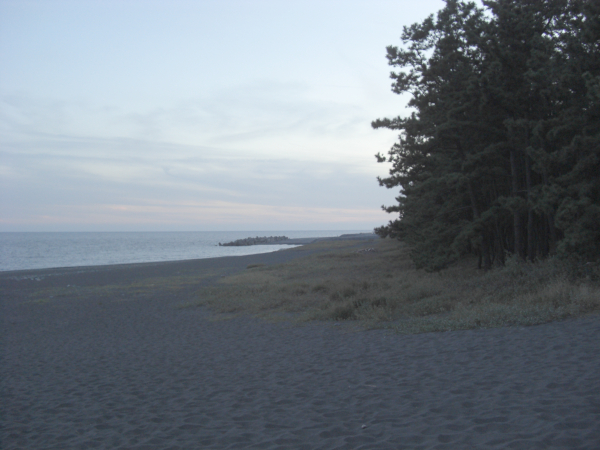
\includegraphics[width=1\textwidth]{ARKA/tier.jpg}
\end{figure}

\emoji{x_knoos}
顺便问一下,Lein,我们现在看的是那片海啊?


\emoji{l_iks}
阿这,我们,在,在,在首都Arna南边,边,边的,的Kateej...(´·ω·`)


\emoji{x_pilp}
其实就是静冈县 :-7


\emoji{l_vexl}
诶呀,这是善意的谎言啦\~{}


%``([a-z]+)''
%``$1''



\chapter[副词]{副词}
%\chapter[短标题显示在页面]{长标题显示在目录}

\emoji{l_deyu} 
\hypertarget{chapter-adverb}{我们}上次学习了Arka的时态和体态,紫苑,你还记得吗?


\emoji{x_vesn} 
动词加``-at''变成过去时.对应的,``-or''变成进行形,``-ik''变成完成形.

``写''是``axt,''那么``axtat''就是``已经写了,''而``axtor''意思是``正在写'',``axtik''意思是``写完了.''

英语的进行时和完成时还要加``be''或者``have''之类的,但Arka里面加后缀就行了.

那未来怎么表达呢?像``将要写.''


\emoji{l_niit} 
你应该在动词前面加一个副词, ``sil.''

``Axt sil''意思是``将要写.''跟``-at''不一样,``sil''不是后缀,所以不要写成``axtsil,''而应该写``axt sil.''


\emoji{x_niit} 
``Axtat'' (写过了)比``axt sil'' (将要写)要短呢.

这是为什么呢?


\emoji{l_sena_deyu} 
好问题!因为过去时出现得更加频繁.

过去时,进行时,和完成时比较短是因为它们出现的更频繁.不常出现的时态就用``sil''之类的副词表达.

这些是Arka的其他副词.我把常用的副词打成表:
\begin{table}[h!]

    %\caption{常用副词}
    \begin{tabular}{|c|c|c|} % {l|c|r}<-- Alignments: 1st column left, 2nd middle and 3rd right, with vertical lines in between
      \hline
	  \textbf{词汇} & \textbf{简要翻译} & \textbf{意义}\\
      \hline
      lax&  想要做&  希望\\\hline
  	van&  要做&  意志\\\hline
  	sen&  能&  可能性\\\hline
  	vil&  不能&  没有可能性\\\hline
  	das&  为什么不&  提议\\\hline
  	fal&  必须&  义务\\\hline
  	flen&  可以&  许可\\\hline
 	xiit&  让我们&  劝诱\\\hline
  	yu&  被&  被动\\\hline
    \end{tabular}

\end{table}    

\emoji{x_asex} 
Arka的副词相当便利呢.像英语之类的,助动词先得一堆.

当你表达``想要'',只需要加上``lax'',``为什么不''只要用``das''时,那可舒服了.

另说一下,这些都能是动词吗.我是说,一般的动词都像``高高地''或者``猛烈地'',这样.


\emoji{l_sena} 
``强,猛''是 ``vien'',``猛烈地''是 ``vienel.''要把形容词变成动词,你只需要加``-el''后缀就行了.

Arka有两种副词,一种想辅助词一样的,和形容词加``-el''转化来的.

结尾是元音的,就不加``-el'',而是加``-l''.``aalo''意思是 ``灵巧,''那么``灵巧地''就是``aalol,''而不是``aaloel.''

来个小练习,``紫苑可以写Arka''要怎么说?
%dexterous:灵巧

\emoji{x_lo} 
``xion axt sen arka''?


\emoji{l_ket} 
嗯~,对了!♪


\emoji{x_knoos} 
嘿, 我在表里找到了``被动语态''呢.这是啥?


\emoji{l_diina} 
``yu''产生被动语态. ``xion axt arka''意思是``紫苑写Arka,''这是主动语态.

要把它变成被动语态,就--\\
\textbf{
\quad1) 在动词后面加``yu'': xion axt yu arka\\
\quad2) 把主语和宾语倒过来: arka axt yu xion}

--就这样.

``arka axt yu xion''意思是``Arka被紫苑写.''


\emoji{x_loki} 
OK,Arka不用加``be,''我也费不上记动词的过去分词.只要加``yu'',然后被主宾关系倒过来就行了.

我逐渐地能写复杂的句子了呢.

但是我还不能翻译``这是一个苹果.''
Lein老师,你下次会教我Arka的系动词吧(\FiveStar ω\FiveStar)


%``([a-z]+)''
%``$1''



\chapter[系动词]{系动词}
%\chapter[短标题显示在页面]{长标题显示在目录}

  

\emoji{x_sena} 
呐, Lein,这是啥?

\begin{figure}[H]

\includegraphics[width=0.7\textwidth]{ARKA/ket.jpg}
\end{figure}

\emoji{l_ket} 
猫!

喵喵\~{}.

我之前给你说,猫在Arka里叫做``ket''.

``这是猫'',就说``tu et ket.''


\emoji{x_niit} 
Arka里注释在最前面呢,所以``tu''就是``这个,'' ``et''意思是``是.''


\emoji{l_asex_kal} 
对,``et''是系词.``tu et oma''意思是``这是一只狗.''


\emoji{x_lo} 
``oma''的地方可以填形容词吗?


\emoji{l_sena_deyu} 
可以.``tu et kai''意思是``它很大.''


\emoji{x_loki} 
变过去式就加``-at'',对吧?

那么``它之前很大''就是``tu etat kai''吗?


\emoji{l_pels} 
不是的,应该说``tu at kai.''

系词出现得相当频繁,所以我们不说``at''而是说``etat.''

这对``or''(进行时)和``ik''(完成时)也适用.

``tu or kai''意思是``它正在长大,''而``tu ik kai''意思是``这已经长大了.''


\emoji{x_tisse} 
哈哈,这样我也不用记``was''或者``been''这类的分词了.

Arka的系动词就是``et.'' ``tu et miik''意思是``这是一个苹果.''

句子的顺序就和``xion axt arka'' (紫苑写Arka)一样呢.记得住记得住.

顺带一说,``紫苑不写Arka''和``紫苑写Arka吗?''应该怎么说?


\emoji{l_nax} 
你是说疑问句和否定句吗?

OK,我下次就教你.



%``([a-z]+)''
%``$1''



\chapter[疑问句,否定句]{疑问句,否定句}
%\chapter[短标题显示在页面]{长标题显示在目录}

  



\emoji{l_diina}
这是我前几天在公园散步时看见的花.

紫苑,这是樱花吗?
\begin{figure}[H]
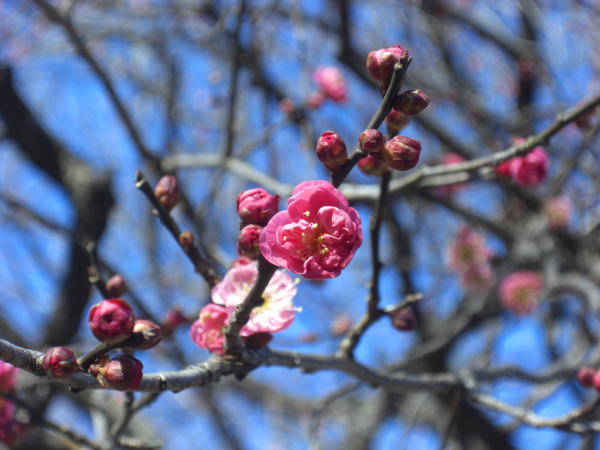
\includegraphics[width=0.7\textwidth]{ARKA/ping.jpg}
\end{figure}

\emoji{x_lo}
额,这是梅花,不是樱花哟

呐,在Arka里怎么说"这是梅花."?

\emoji{l_asex_kal}
"这是梅花"应该说"tu et ping"。"tu et"就是上次讲过的

"这是樱花"也差不多,说"tu et seron"。

"这是樱花吗"就在句子最后加上mia."tu et seron mia?"

不过很多场合我们不特意加"mia",只是在句子后面加一个问号.


\emoji{x_pil}
疑问的时候语调要上扬一些呢.
相比于英语的"Do you...?"Arka要简单呢。跟汉语在句末加"吗"比较像.


\emoji{l_sena}
另一方面,"这不是樱花"应该说"tu de seron".
de一个词就表示系动词的否定,像是"isn't"一样.
顺便一说,女生不用"de",而用"te".


\emoji{x_niit}
那么我其实应该说"tu te seron"吗.

%ともあれ、「~でない」はdeね。「~DEない」と覚えようw ------翻译不过来的梗
另外,"不写"应该怎么说呢?


\emoji{l_xanxa}
be动词以外嘛,就在动词前面放副词"en".

axt是"写"、那么"en axt"就是"不写".


\emoji{x_demo}
哦......"紫苑不写Arka"就是"xion en axt arka"吧。

让我总结一下:

\textbf{
疑问句:只是在句尾加"mia"\\
否定句:be换成de,另外就是在动词前面加"en".
}

\emoji{l_deyu}
最后来做个小测试吧.

试着写下"这是猫吗?","这不是猫,是狗.","紫苑会写Arka吗?"这三个句子
答案就在下回的开头.atte!(加油!)




%``([a-z]+)''
%``$1''



\chapter[祈使句]{祈使句}
%\chapter[短标题显示在页面]{长标题显示在目录}

 
\emoji{l_asex_kal} 
我们上次学了Arka的疑问句和否定句
紫苑,你把作业做的咋样了?


\emoji{x_pels} 
"它是猫吗?"; tu et ket mia?

"它不是猫,它是狗"; tu de ket. tu et oma.

"紫苑不写Arka吗?"; xion en axt arka mia?

--对吧?


\emoji{l_ket} 
OK,好样的!

最后一个句子是疑问句和否定句的组合,看起来你也做得不错呢.


\emoji{x_fron} 
副词"en,"后面接上动词表示否定.在英语里,类似的词"not,"出现在动词后面.

Arka里形容词在动词后面,但是"en"却在动词前面.这有点奇怪.

还有其他在动词前面的词吗?


\emoji{l_asex_kal} 
有,我接下来教你Arka的祈使句.

你要表示祈使,就在动词前面放"re"."re lef"意思是"跑!"

我给你把出现在动词前面的词列成表
\begin{table}
    \begin{tabular}{|c|c|c|} % {l|c|r}<-- Alignments: 1st column left, 2nd middle and 3rd right, with vertical lines in between
      \hline
	  \textbf{词汇} & \textbf{简要翻译} & \textbf{意义}\\
      \hline
      re&  做&  命令\\\hline
  mir&  请做&  要求\\\hline
  den&  不准&  禁止\\\hline
  fon&  请不要&  劝阻\\\hline
    \end{tabular}
\end{table}

\emoji{x_lo} 
"请不要写"是"fon axt."

你怎么说"请不要走"或者"请过来"?


\emoji{l_deyu} 
"fon ke"和"mir luna."

"ke"是"走,"然后"luna"意思是"来."


\emoji{x_asex} 
明白了.

这意味着祈使句可以向英语和汉语一样省略主语.

"you come here"也可以是"come here."


\emoji{l_sena} 
这个省略不必强求.

"ti mir luna"就像"你过来一下."


\emoji{x_tisse} 
在Arka里"You"是"ti"吗?

说到"你," 我还没有在Arka里学到"我","他"之类的代词呢.


\emoji{l_iks} 
唔...

\emoji{x_knoos} 
嗯?


\emoji{l_hik} 
其实我一直在......故意避免它们......


\emoji{x_knoos} 
为啥?


\emoji{l_reiv} 
因为真的很烦......(´·ω·`)





%``([a-z]+)''
%``$1''



\chapter[代词]{代词}

%\chapter[短标题显示在页面]{长标题显示在目录}

\emoji{l_diina} 
\hypertarget{chapter-pronouns}{来},我来教你Arka的代词,像``我'',``你'',``他'',``它''.


\emoji{x_seernik} 
你上次不是说它很复杂吗?先拣主要的说吧.

首先,无生命物的代词是什么?我是说, ``这个,'' ``那个'' and ``他.''


\emoji{l_asex_kal} 
``这个''是``tu,''``那个''是``le.''

我们没有``它.''


\emoji{x_lo} 
OK, ``tu''和``le.''啊,你之前教过我``tu.''
那像``我''这样有生命物的代词呢?


\emoji{l_niit} 
``我''是``an'', ``你''是``ti.''

``他''和``她''都是``lu.'' ``lu et xion''意思是``她是紫苑.''

``lu''意指这个人离说话人近,而``la''意指这个人离说话人远.


\emoji{x_loki} 
那就是说``lu''是``这个人,''而``la''是``那个人.''

``她/他''是一样的,但是``lu''和``la''却有区分.

与``tu''和``le''的区别就在于有生命.

还行吧,现在Arka大代词还没什么奇怪的地方.

\emoji{x_tisse} 
哦哦,明白了.有``I,'' ``my,'' ``me'' and ``mine''\footnote{此处为英语原文的例子,日语原文是「私が」「私の」「私を」「私のもの」}
等等的区别,就像英语和德语那样,对吧?


\emoji{l_deyu} 
不不不,Arka只有``我''和``我的''.
``Me''和``I''都是``an,''而``my''和``mine''都是``ant.''
代词的种类只有两种:``我'' 和 ``我的,'' ``你'' 和 ``你的,'' ``他\\她'' 和 ``他\\她的.''我给你列个表:
\begin{table}[H]
    \begin{tabular}{|c|c|c|c|} % {l|c|r}<-- Alignments: 1st column left, 2nd middle and 3rd right, with vertical lines in between
    \hline
	我&  an&  我的&  ant\\\hline
	你&  ti&  你的&  tiil\\\hline
  	他/她(近)&  lu&  他/她(近)的&  luut\\\hline
	他/她(远)&  la&  他/她(远)的&  laat\\\hline
	这个&  tu&  这个的&  tuul\\\hline
	那个&  le&  那个的&  leet\\\hline
	\end{tabular}
\end{table}

\emoji{x_pil} 
右边的看起来都以``l''或者``t''结尾.

也许他们确实不规则,不过总比英语的``I,'' ``my,'' ``me'', ``mine''要好些.其实也不难.


\emoji{l_iks} 
我刚才列出的代词是最普通的.

我给你说过,女生用否定系动词的时候不用``de''而是用``te''.

Arka的代词用法有很多种.明确谁在说,谁在听,作用很大.
根据说话者的不同,代词也有不同.你看下面这个表,女生倾向于用这些代词.
\begin{table}[H]
    \begin{tabular}{|c|c|c|c|} % {l|c|r}<-- Alignments: 1st column left, 2nd middle and 3rd right, with vertical lines in between
    \hline
	我&  \textcolor{pink}{non}&  我的&  \textcolor{pink}{noan}\\\hline
	你&  \textcolor{pink}{tyu}&  你的&  \textcolor{pink}{tuan}\\\hline
  	他/ 她(近)&  lu&  他/ 她(近)的&  luut\\\hline
	他/ 她(远)&  la&  他/ 她(远)的&  laat\\\hline
	这个&  tu&  这个的&  tuul\\\hline
	那个&  le&  那个的&  leet\\\hline
	\end{tabular}
\end{table}

\emoji{x_loki} 
这样啊.人与人之间用的代词确实不一样呢
但是仔细一看,只有``我,'' ``我的,'' ``你''和``你的''有变化呢.


\emoji{l_hik} 
像你这样的女生喜欢自称``non,''但是其他类型的会叫``yuna''或者``noel.''

男生也用好多代词,甚至中性的人类和有灵魂的非生命体也有自己的代词.总共有\textcolor{pink}{12}种代词.

另外,Arkaz最大的挫折就在\hyperlink{appendix-pronouns}{这个代词表}......


\emoji{x_nik} 
?Σ(°ロ°;)

每个人和每个人的代词都不一样...! 但是在区别说话者的个性时非常有用.


\emoji{l_pels} 
每个代词都有复数形式,``我们''是``ans,''``我们的''是``antes''.

当然,这些复数形式也因人而异.性格内向的萌妹子会用``lena'' (我们)和``lenan'' (我们的).


\emoji{x_iks} 
OK,我,服了.这,就,是,代,词.(;\CircleShadow ω \CircleShadow )ゞ


\emoji{l_diina} 
确实是.不过你平时只要记住``an行''和``non行''就行了.不用全记住的.

不过,你刚才也说了,多亏了这些多彩的代词,Arka可以鲜明地表示人物性格.


\emoji{x_asex} 
辞藻华丽呢.


%``([a-z]+)''
%``$1''



%\part{La Mondo kiel Volo}
% \include{./TeX_files/chapter07}
% 插入参考文献、致谢等
\appendix
\chapter[Arka的所有代词]{Arka的所有代词}
%\chapter[短标题显示在页面]{长标题显示在目录}
Arka的位相受到「个性位相、方言位相、环境位相、关系位相」四种要素约束,下面是10种
\footnote{
不止10种,注意下面的表,英语版的表没有[xia]一行,而是把[milia]一行当做[女-可爱]的代词序列.并且英语版没有方言,环境,关系等位相的描述,这里以日语版为准.
下面注明每种性格的时候,也没有提到[xia].
}
位相的表.
\section{个性位相}
\begin{table}[H]
	\centering
   	
\resizebox{\textwidth}{!}{\begin{tabular}{|c|c|c|c|c|c|c|c|c|c|c|c|c|c|c|} % {l|c|r}<-- Alignments: 1st column left, 2nd middle and 3rd right, with vertical lines in between
   	\hline
   性别&  性格&  位相名&  我&  我的&  我们&  我们的&  你&  你的&  你们&  你们的&  确认&  不确认&  传达& 日语译例
   \footnote{英语表中无相关译例,译者尝试用汉语重建译例,
   然而汉语的代词常用的是在太少,即使做出来了,很多都会有重复,参考作用不会太大,所以没有做.大家看日语版译例,可知一二
   }
   \\\hline
   man&  常规&  seet&  an&  ant&  ans&  antes&  ti&  tiil&  tiis&  tiiles&  kok&  sei&  tisee&私\\\hline
   man&  强壮&  arden&  der&  dent&  orfen&  orfant&  dis&  din&  sedis&  sedin&  kaak&  daana&  dizmal&俺\\\hline
   man&  粗鲁&  alben&  dai&  daid&  cuud&  cuudis&  baz&  bazel&  bcand&  bcendi&  daxxa&  zor&  laga&オレ\\\hline
   man&  智性&  yuul&  ami&  amit&  sean&  seant&  tol&  tolte&  flent&  flandol&  ranxel&  fixet&  flenzel&僕\\\hline
   man&  草食&  pikko&  men&  menal&  liia&  liian&  sala&  salen&  setyu&  setut&  xatta&  sivan&  ramma&ぼく\\\hline
   女&   强势&   amma&   ema&   emil&   polte&   polton&   twa&   twal&   klans&   klansen&   soona&   yundi&   weeze&   アタシ\\\hline
   女&   明朗&   mayu&   noel&   notte&   xenon&   xenoan&   xian&   xiant&   telul&   telet&   sanna&   enxe&   xiima&   あたし\\\hline
   女&   胜气&   gano&   gan&   ganet&   kalas&   kaldes&   beg&   beget&   walet&   wolden&   yatte&   indi&   belze&   ウチ\\\hline
   女&   绮丽&   yunk&   yuna&   yunol&   kolet&   ekol&   moe&   moen&   felie&   felial&   axem&   tuuyu&   linoa&   私\\\hline
   女&   中立&   milia&   non&   noan&   lena&   lenan&   tyu&   tuan&   lilis&   lilin&   sete&   eyo&   tisse&   わたし\\\hline
   女&   可爱&   xia&   xia&   txia&   xiif&   xifet&   myu&   myuan&   milis&   milin&   tanya&   poyo&   yuwa&   わたし\\\hline
   中性&    &solferj&  noa&  noett&  lenoa&  lenoan&  tiam&  tiamet&  letiam&  letiant&  kotta&  ansem&  sante&私\\\hline
   精灵&   & kotan&  nana&  nanatu&  nanasse&  nanassetu&  mina&  minatu&  minasse&  minassetu&  nano&  milei&  sian&ワタシ\\\hline
    \end{tabular}}
\end{table}
以性别和性格为基础分解,有12种位相.

男性有seet, arden, alben, yuul, pikko,默认情况是seet.

女性有amma, mayu, gano, yunk, milia。女性没有默认情况,根据性格决定位相,看心情有时候也用其他位相.
在公共场合发言时女性也可以用seet.个人对话时女性往往用yuul.
总之女性有很多选择.这一边女性既可以穿裤子也可以穿裙子,女性专用车厢和普通车厢都可以乘坐,像日本一样。

中性代词是Yult,Lyuu这样中性感的人物使用的.所谓"草食","男の娘"
\footnote{我很好奇他们是不是真的愿意明显地表示出来.也许这种勇气,和容许这种勇气的氛围,只在Kaldia存在吧}之人也适用。
相反,不像女性的中性女性也会使用,而不会表现"胜于男性"的气场.要不然就不用amma, mayu, gano,而直接用男性的代词了。

精霊代词是那些无生命者所用的.像付丧神或者凭依的思念体.

以下是大致的10类代词的解释.这个标准保证不论什么样的人都有合适的选择。傲娇之类易怒的女生会用mayu.
在孩子眼里长辈很多,于是使用pikko的场合也很多.同样的幼女会更多用yunk, milia.

seet:男性默认

arden:肉食男子、体育会

alben:粗野

yuul:智性

pikko:草食男子同样也做男性敬体

amma:大姐大,豪快,胜过男性

mayu:元气,明朗

gano:剩气,刚强

yunk:华丽系

milia:可爱系

\subsection{敬体}

男性用pikko与长辈讲话,女性则参考下表.
\begin{table}[H]
    \begin{tabular}{|c|c|c|c|c|c|c|c|c|c|c|} % {l|c|r}<-- Alignments: 1st column left, 2nd middle and 3rd right, with vertical lines in between
      \hline
      我&     我的&       我们&     我们的&     你&     你的&  你们&     你们的&     确认&  不确认&  传达\\\hline
      meid&   meiden&     xelis&  xelien&  halka&  halkan&  isfel&  isfelia&  malia&  nyannya&  yuulia\\\hline
  \end{tabular}
\end{table}

\subsection{第三人称}


第三人称只有mayu, yunk, milia是特别的,用法中特别的也只占一小部分.
\begin{table}[H]
    \begin{tabular}{|c|c|c|c|c|c|c|c|c|} % {l|c|r}<-- Alignments: 1st column left, 2nd middle and 3rd right, with vertical lines in between
    \hline
    seet&  luus&  luutes&  laas&  laates&  tuus&  tuules&  lees&  leetes\\\hline
     mayu&  \textcolor{red}{luan}&  \textcolor{red}{luant}&  \textcolor{red}{lain}&  \textcolor{red}{laint}&  tuus&  tuules&  lees&  leetes\\\hline
     yunk&  \textcolor{red}{luan}&  \textcolor{red}{luant}&  \textcolor{red}{lain}&  \textcolor{red}{laint}&  \textcolor{red}{tutu}&  \textcolor{red}{tutul}&  \textcolor{red}{lele}&  \textcolor{red}{leent}\\\hline
     milia&   \textcolor{red}{luan}&  \textcolor{red}{luant}&  \textcolor{red}{lain}&  \textcolor{red}{laint}&  \textcolor{red}{tutu}&  \textcolor{red}{tutul}&  \textcolor{red}{lele}&  \textcolor{red}{leent}\\\hline

  \end{tabular}
\end{table}

\subsection{千金位相}

被称为大小姐的阶层在yunk, milia, mayu的任意一个位相像前面加上an.
例如anyuna.敬体在使用meid系列时也会在前面加上an,像anmeid.
这是装腔作势的贵族和有钱人的说法,虽然在现实中不太常见,但也不是零。动画和漫画在塑造大小姐角色时也会用到.
至于听起来像不像装腔作势的讨厌大小姐,取决于本人的性格和对方的接受方式。是讨厌,或是装腔作势,或是真正的大家闺秀,视情况而定。

anyuna yuus fan anmoe luna ankolet anlinoa(你我也许会相处甚欢
\footnote{英语:You may join us.日语:あなた、わたくしたちに混ぜてさしあげてもよくてよ.真的,我翻不准.
}
).

一直说an的做法被嘲为anankuom(anan语气),这么做会让你看起来像个马鹿.

再者,第三人称也加这个an,像anluan, antutu之类。

\subsection{位相的使用方法}


根据关系和语境切换位相是很常见的.例如对晚辈an使用der,对长辈则使用men.这和日语里不要对长辈使用"俺"是一个道理.
不过也有真的不换位相的人.就像有对长辈说"俺"之类粗话的人一样.

第一人称用ami而第二人称用dis也可以,这被叫做位相的交叉.
"我(僕)"是ami,对方根据与自己的关系,有时会变成"你(tol)",有时会变成"你(dis)\footnote{对应的日语分别是「君」和「お前」}"。
这和日语里用"僕"自称,但对别人称"君","あなた""お前"是一样的.
不过,自称am而对对方称tol是默认情况.同样的,自称der,称对方dis也是默认的.

\subsection{单词位相}

女性一般用xen(饮)代替kui(食べる).这时根据位相的不同,遣词也会变化.
举以下几个例子.这些单词在词典中多带有[rente],[郑重]等标签。

动词

kui→xen
ku→rens
mok→xidia
skin→fians

名词

xia→felver

形容词

vein→fein

副词

lax→lan
ris→rin
van→fan

格词

fin→fien

\section{方言位相}

在Arbazard同一片大地上Arsia使用西方方言,Kadesh使用南方方言,Arbazard使用北方方言.
每一处的语言都无疑是Arka,但语言学上将其按方言位相区分.


\section{环境位相}

根据身份和立场,语言也有不同.
同样的含义,由教师说出和由母亲说出就不一样.
公共场合就使用正规的文法,减少剧中的省略.同样的遣词也偏向于seet系.

\section{关系位相}
关系位相由彼此的环境相互决定.
关键是说话人的环境不会改变。

Lidia→Yult:"leen yultan, lax piyo nono?(呐,Yult,想要我们的小鸡雏?)
Lidia→Seren:"nee seren sou, tyu lax mive noan?"(啊,Seren君,要小鸡雏吗?
\footnote{原文分别是"ねーぇ、ユルトちゃん、あたちのぴよちゃんほしい?","あ、セレン君、ひよこ要る?"
}?)

%``([a-z]+)''
%``$1''

\backmatter
% bibliography, glossary and index would go here.
\end{document}
% \begin{titlepage}	
% % 封面信息
% 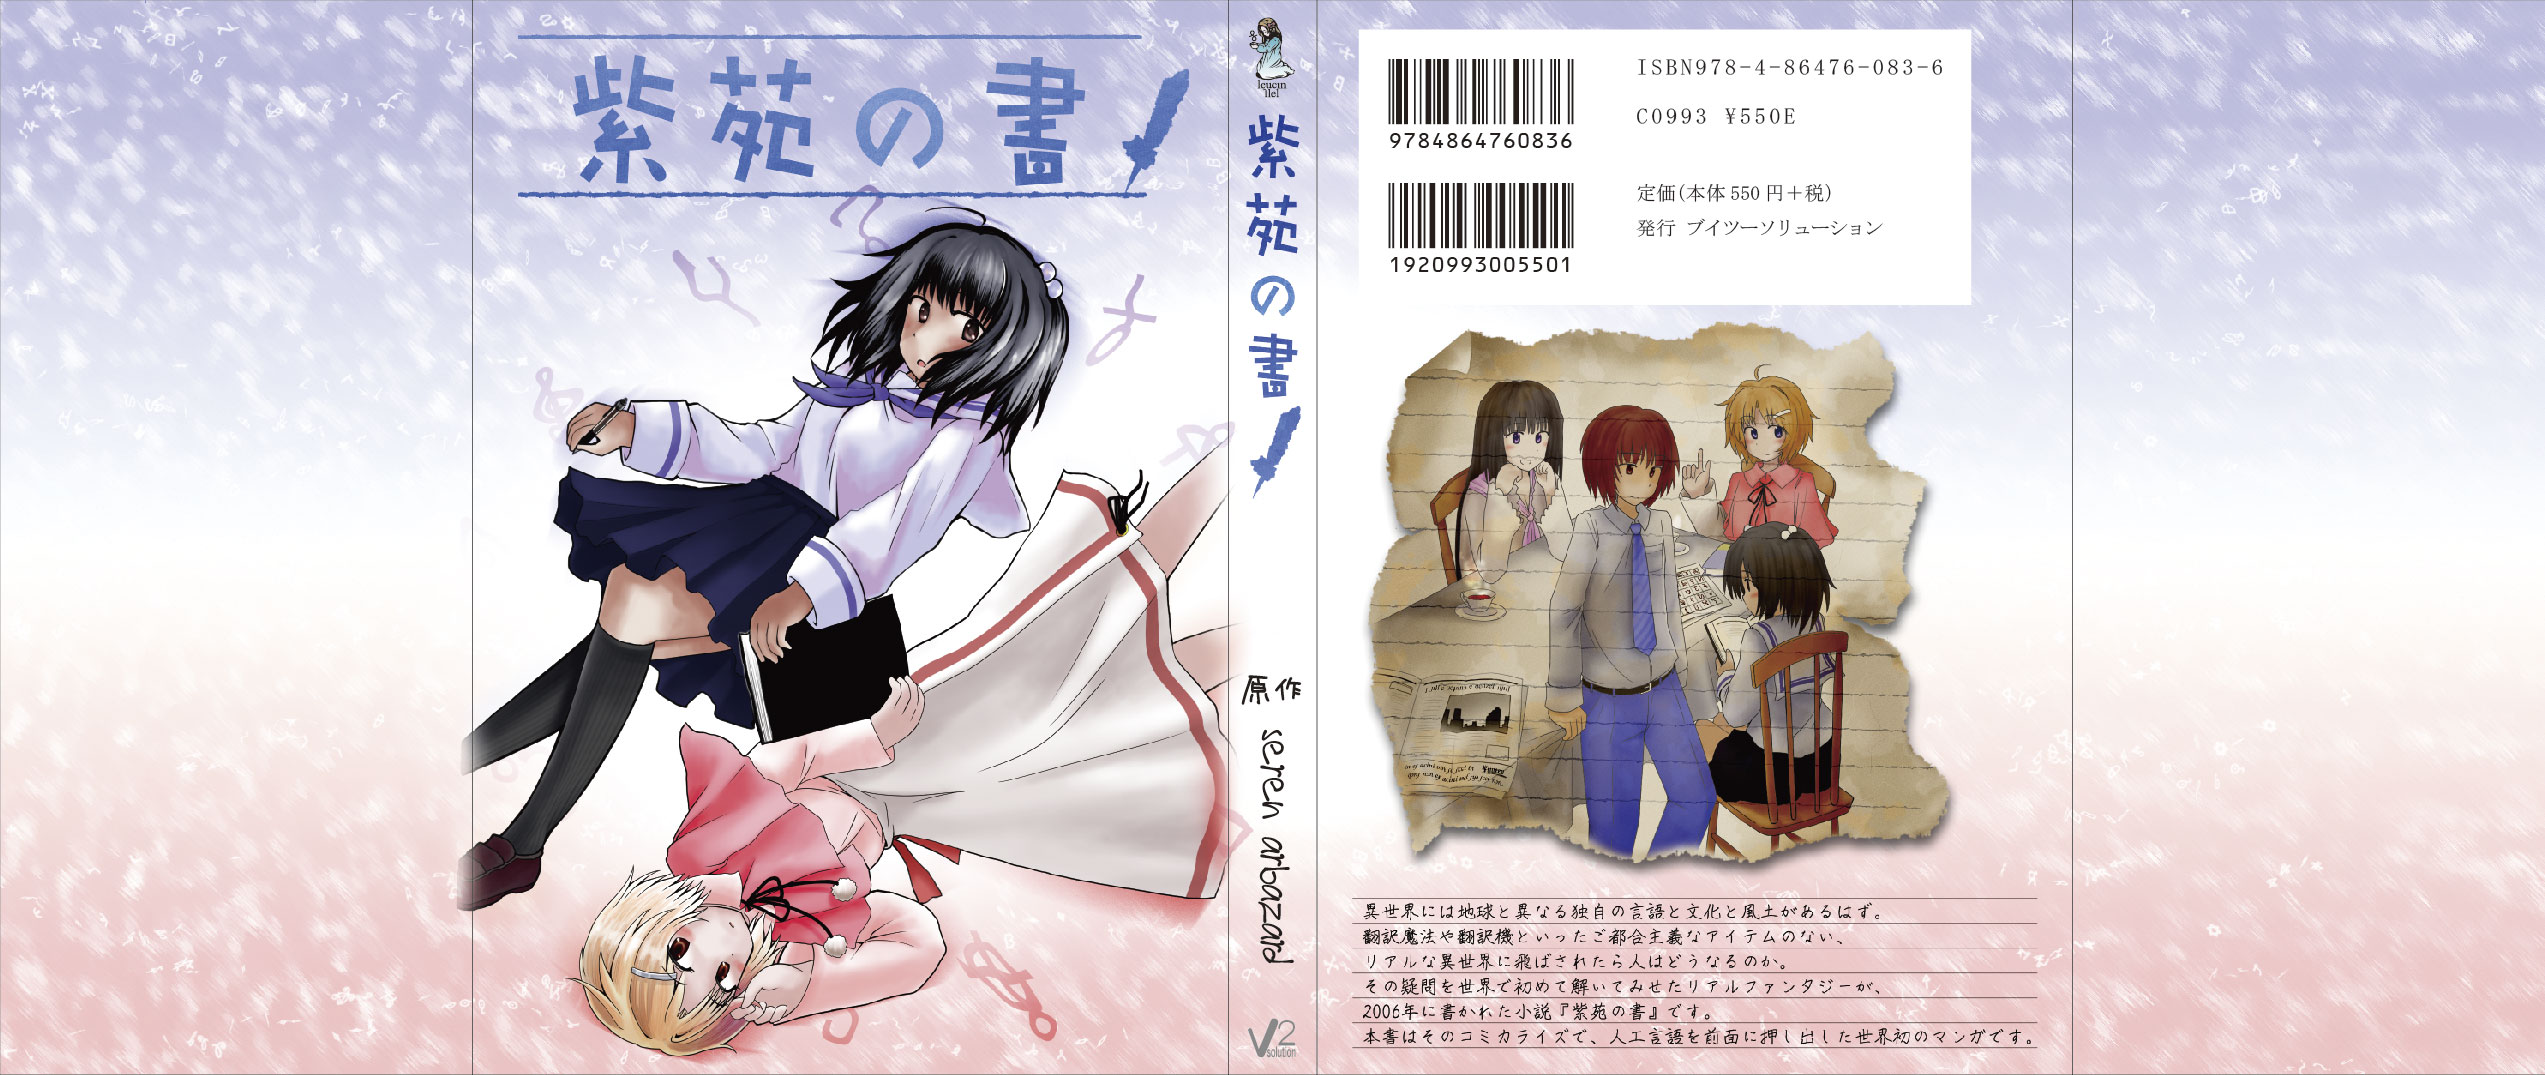
\includepdf[pages={1}]{cover.pdf} %曲线救国的思路,外界自建封面,然后调用
% \end{titlepage}